\documentclass[twocolumn]{article}

\usepackage[utf8]{inputenc}
\usepackage[T1]{fontenc}
\usepackage[french]{babel}
\usepackage{geometry}
\usepackage{amsmath,amssymb}
\usepackage{booktabs}
\usepackage{graphicx}
\usepackage{microtype}
\usepackage{caption}
\usepackage{float}
\usepackage[numbers,sort&compress]{natbib}
\usepackage[colorlinks=true, linkcolor=blue, citecolor=blue, urlcolor=blue]{hyperref}

\geometry{
  a4paper,
  top=2cm, bottom=2.5cm,
  left=1.5cm, right=1.5cm,
  columnsep=0.8cm
}

\graphicspath{{figures/}}

\title{\textbf{Profils d'élèves décrocheurs en mathématiques}\\
\large Analyse non supervisée et supervisée sur le dataset \textit{Student Alcohol Consumption}}
\author{Mathéo Gros \and Maël Lozac'h \and Mathieu Piekarz}
\date{Juin 2026}

\begin{document}

\maketitle

\begin{abstract}
Nous analysons le jeu de données \textit{Student Alcohol Consumption} pour identifier des profils d'élèves susceptibles de décrocher en mathématiques en cours d'année. Le décrochage est défini comme l'obtention d'un G3 nul alors que G1 est positif~; il touche 9,6\,\% des 395 élèves du dataset mathématiques. Après sélection de 8 variables socio-comportementales discriminantes, une analyse factorielle sur tableau de distances (AFTD) suivie d'un clustering (CAH-Ward et $K$-means) permet d'identifier 4 profils d'élèves. Leur lien avec le décrochage est ensuite évalué statistiquement et par apprentissage supervisé.
\end{abstract}

\section{Introduction}

Le jeu de données provient d'une enquête conduite dans deux lycées portugais~\cite{cortez2008}. Il recense 395 élèves en mathématiques et 649 en portugais, avec leurs notes trimestrielles (G1, G2, G3) et une trentaine de variables socio-démographiques et comportementales. Notre problématique est la suivante~: dans quelle mesure ces variables, disponibles en début d'année, permettent-elles d'identifier des profils d'élèves susceptibles de décrocher en mathématiques~?

Le rapport est organisé en trois parties. La section~\ref{sec:prelim} définit le phénomène de décrochage et sélectionne les variables explicatives. La section~\ref{sec:unsupervised} construit une distance mixte, applique une AFTD et identifie quatre profils par clustering. La section~\ref{sec:validation} teste statistiquement le lien entre ces profils et le décrochage, puis évalue des classifieurs supervisés. La conclusion synthétise les résultats et les limites de l'étude.

\section{Analyse préliminaire et sélection des variables}
\label{sec:prelim}

\subsection{Identification du phénomène de décrochage}

L'examen de la distribution des notes finales G3 révèle un pic anormal à G3\,=\,0 en mathématiques (9,6\,\% des élèves, contre 2,3\,\% en portugais). Un test de comparaison de proportions~\cite[Ch.\,10, \S\,10.4]{polySY02} confirme que cette asymétrie est très hautement significative ($z = 5{,}22$, $p < 0{,}001$). Le phénomène est donc matière-spécifique.

Tous les élèves avec G3\,=\,0 avaient une note G1 strictement positive (G1 moyen\,: 7,5/20), ce qui exclut un absentéisme originel et confirme un abandon en cours d'année. La variable cible est ainsi définie~:
\[
\texttt{decrocheur} = \mathbf{1}[G3 = 0 \text{ et } G1 > 0].
\]

\begin{figure}[h]
\centering
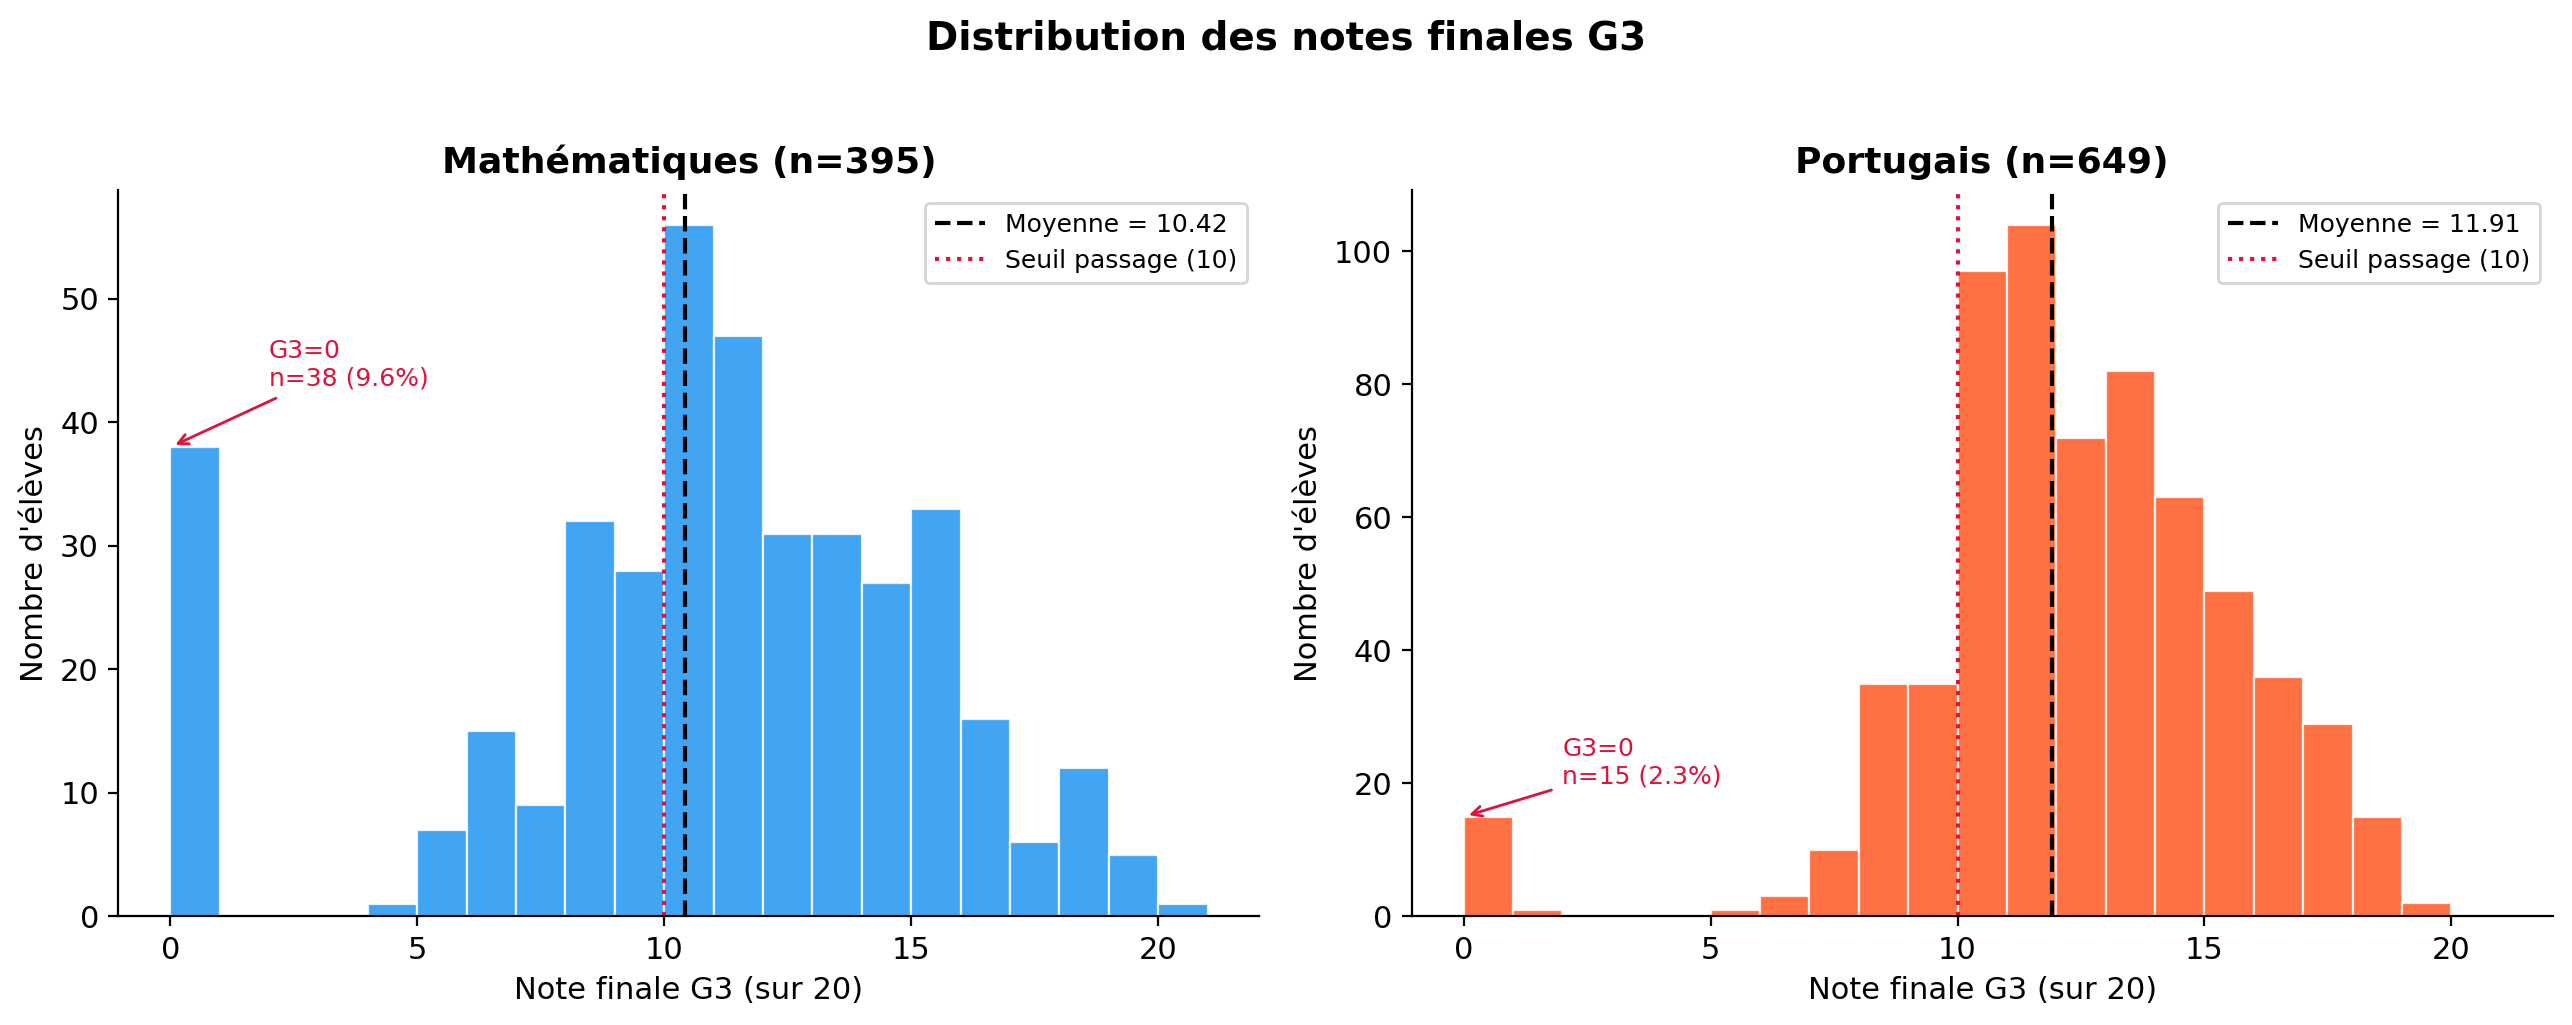
\includegraphics[width=0.95\columnwidth]{00_g3_distribution.png}
\caption{Distribution de G3 en mathématiques et en portugais~; pic à G3\,=\,0 en maths.}
\label{fig:g3}
\end{figure}

\subsection{Sélection des variables}

Les 38 décrocheurs sont comparés aux 357 non-décrocheurs sur l'ensemble des variables disponibles. Pour les variables numériques, le test de Wilcoxon-Mann-Whitney~\cite[Ch.\,10, \S\,10.5.2]{polySY02} est utilisé~; pour les variables catégorielles, le test du $\chi^2$ d'indépendance~\cite[Ch.\,12, \S\,12.1]{polySY02}. Le seuil est fixé à $\alpha = 0{,}10$ plutôt que $0{,}05$~: le faible effectif de décrocheurs ($n=38$) limite la puissance des tests.

La variable \texttt{absences} est écartée malgré sa $p$-valeur $< 0{,}001$~: les décrocheurs affichent paradoxalement 0 absence en moyenne contre 6,3 pour les non-décrocheurs. Ce signal est probablement un artefact administratif (arrêt de comptabilisation après abandon) dont l'interprétation est trop ambiguë pour être retenu. Les 8 variables retenues figurent dans le tableau~\ref{tab:vars}.

\begin{table}[h]
\caption{Variables retenues ($\alpha = 0{,}10$), classées par $p$-valeur.}
\label{tab:vars}
\centering
\small
\begin{tabular}{llr}
\toprule
Variable & Type & $p$-valeur \\
\midrule
\texttt{failures} & quantitative discrète & $< 0{,}001$ \\
\texttt{paid}     & binaire & $0{,}002$ \\
\texttt{higher}   & binaire & $0{,}005$ \\
\texttt{Medu}     & ordinale & $0{,}008$ \\
\texttt{romantic} & binaire & $0{,}014$ \\
\texttt{age}      & quantitative discrète & $0{,}039$ \\
\texttt{Walc}     & ordinale & $0{,}060$ \\
\texttt{schoolsup}& binaire & $0{,}083$ \\
\bottomrule
\end{tabular}
\end{table}

Ces variables dessinent un profil de vulnérabilité cohérent~: échecs antérieurs, moindre capital éducatif maternel, absence de soutien payant et moindre projection vers les études supérieures. Les comparaisons graphiques détaillées sont reportées en annexe~\ref{ann:discriminants} (figure~\ref{fig:ann_discriminants}).

\section{Analyse non supervisée}
\label{sec:unsupervised}

\subsection{Distance mixte et AFTD}

Les 8 variables retenues sont de trois natures~:
\begin{itemize}
  \item \textit{Quantitatives discrètes} (\texttt{failures}, \texttt{age})~: distance normalisée par l'étendue, $d_k(i,j) = |x_{ik}-x_{jk}|/(\max - \min)$.
  \item \textit{Ordinales} (\texttt{Medu}, \texttt{Walc})~: même distance sur rang renormalisé.
  \item \textit{Binaires} (\texttt{higher}, \texttt{paid}, \texttt{schoolsup}, \texttt{romantic})~: désaccord simple, $d_k(i,j) = \mathbf{1}[x_{ik} \neq x_{jk}]$.
\end{itemize}
La distance globale~\cite[Ch.\,2, \S\,2.2]{polySY09} est la moyenne arithmétique des distances partielles~:
\[
d(i,j) = \frac{1}{8}\sum_{k=1}^{8} d_k(i,j) \in [0,1].
\]

Une Analyse Factorielle sur Tableau de Distances (AFTD)~\cite[Ch.\,6]{polySY09} est ensuite appliquée. La distance mixte n'étant pas euclidienne, la matrice doublement centrée $W = -\frac{1}{2}Q_n\Delta^2 Q_n$ présente 375 valeurs propres négatives sur 395~\cite[Ch.\,6, \S\,5.2]{polySY09}~; seules les valeurs propres positives sont retenues pour calculer les coordonnées factorielles. Un seuil de variance cumulée à 58\,\% conduit à retenir 3 axes (inertie cumulée~: 58,1\,\%). La qualité de la représentation est vérifiée par le diagramme de Shepard~\cite[Ch.\,6, \S\,6.2]{polySY09}~: $r = 0{,}901$ et une RMSE de 6,5\,\% de $d_{\max}$, ce qui indique une bonne fidélité aux distances initiales.

\begin{figure}[h]
\centering
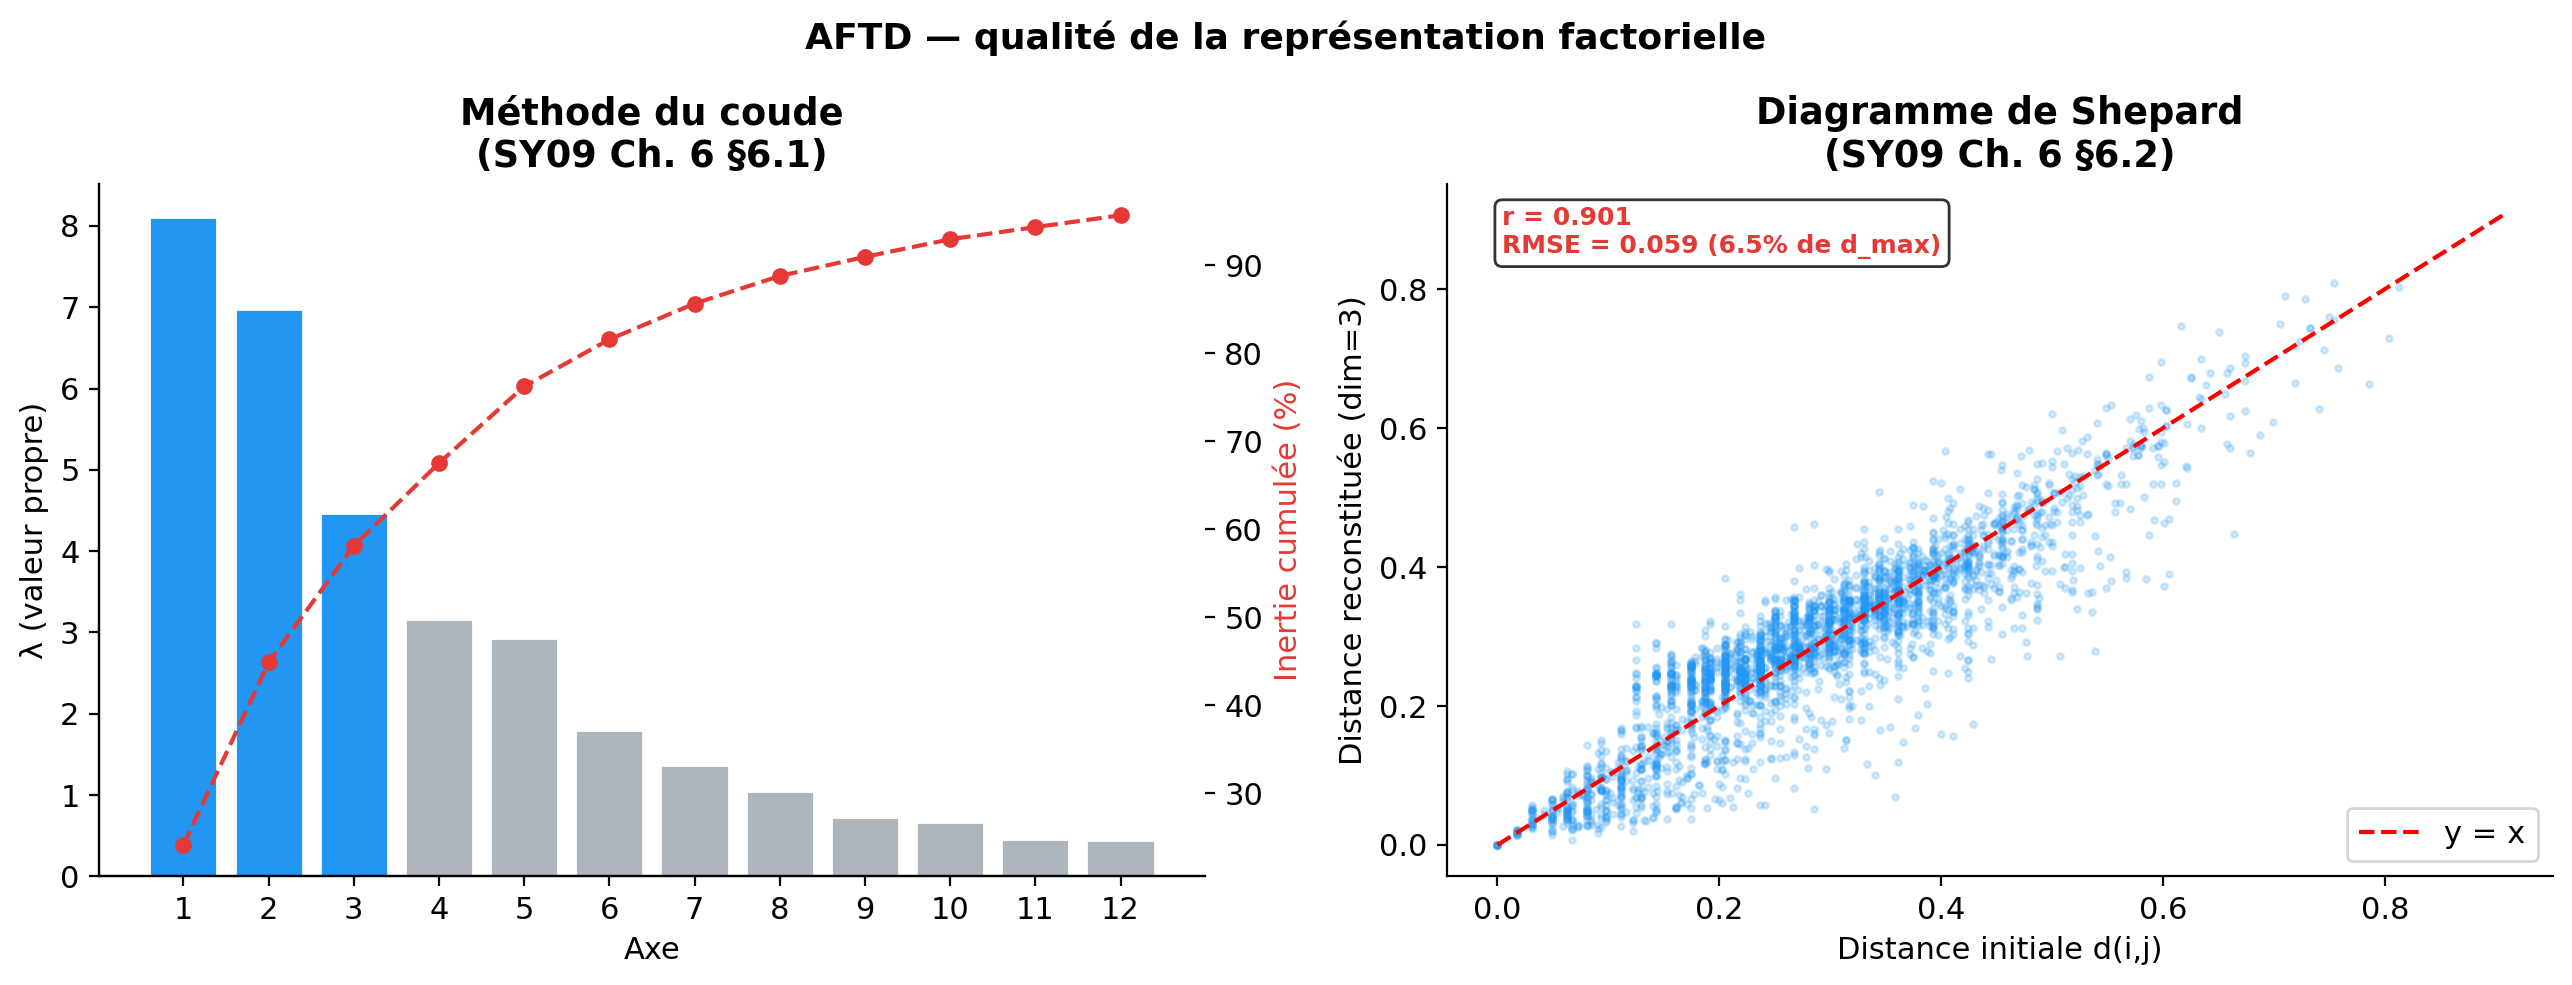
\includegraphics[width=0.95\columnwidth]{03_aftd_scree_shepard.png}
\caption{Scree plot et diagramme de Shepard (AFTD, 3 axes retenus).}
\label{fig:shepard}
\end{figure}

\subsection{Clustering}

Deux méthodes de classification non supervisée~\cite[Ch.\,7]{polySY09} sont appliquées sur les coordonnées factorielles.

\textit{CAH-Ward.} La méthode de Ward~\cite[Ch.\,7, \S\,5.5]{polySY09} est appliquée sur les coordonnées euclidiennes issues de l'AFTD. L'analyse des sauts d'inertie~\cite[Ch.\,7, \S\,4.3]{polySY09} suggère $K=4$ (saut de 0,674 entre $K=4$ et $K=3$)~; le dendrogramme complet est reproduit en annexe~\ref{ann:cah} (figure~\ref{fig:ann_cah}).

\textit{$K$-means.} Le nombre de clusters est sélectionné par le score de silhouette~\cite{inf1421module6} sur l'intervalle $K \in [3, 10]$, qui est maximal à $K=4$. La méthode du coude sur l'inertie intra-classe suggère $K=5$~; la silhouette tranche en faveur de $K=4$ (annexe~\ref{ann:coude_sil}, figure~\ref{fig:ann_coude_sil}).

La concordance entre les deux partitions est mesurée par l'indice de Rand ajusté (ARI)~\cite[Ch.\,7]{polySY09}~: $\text{ARI} = 0{,}980$, ce qui confirme la stabilité de la solution. Une analyse de robustesse par bootstrap (médiane ARI\,=\,1,000 sur des sous-échantillons à 80\,\%) renforce cette conclusion. La suite utilise la partition $K$-means.

\subsection{Description et interprétation des 4 profils}
\label{sec:profils}

Une fois la partition $K=4$ obtenue, les individus sont projetés sur le plan factoriel AFTD (axes 1--2) et colorés selon leur cluster $K$-means (figure~\ref{fig:plan_clusters}). Les décrocheurs sont superposés en étoiles noires~: ils ne forment pas un nuage isolé, mais se concentrent visuellement dans le cluster C1, ce qui préfigure l'analyse des taux de décrochage ci-dessous.

\begin{figure}[h]
\centering
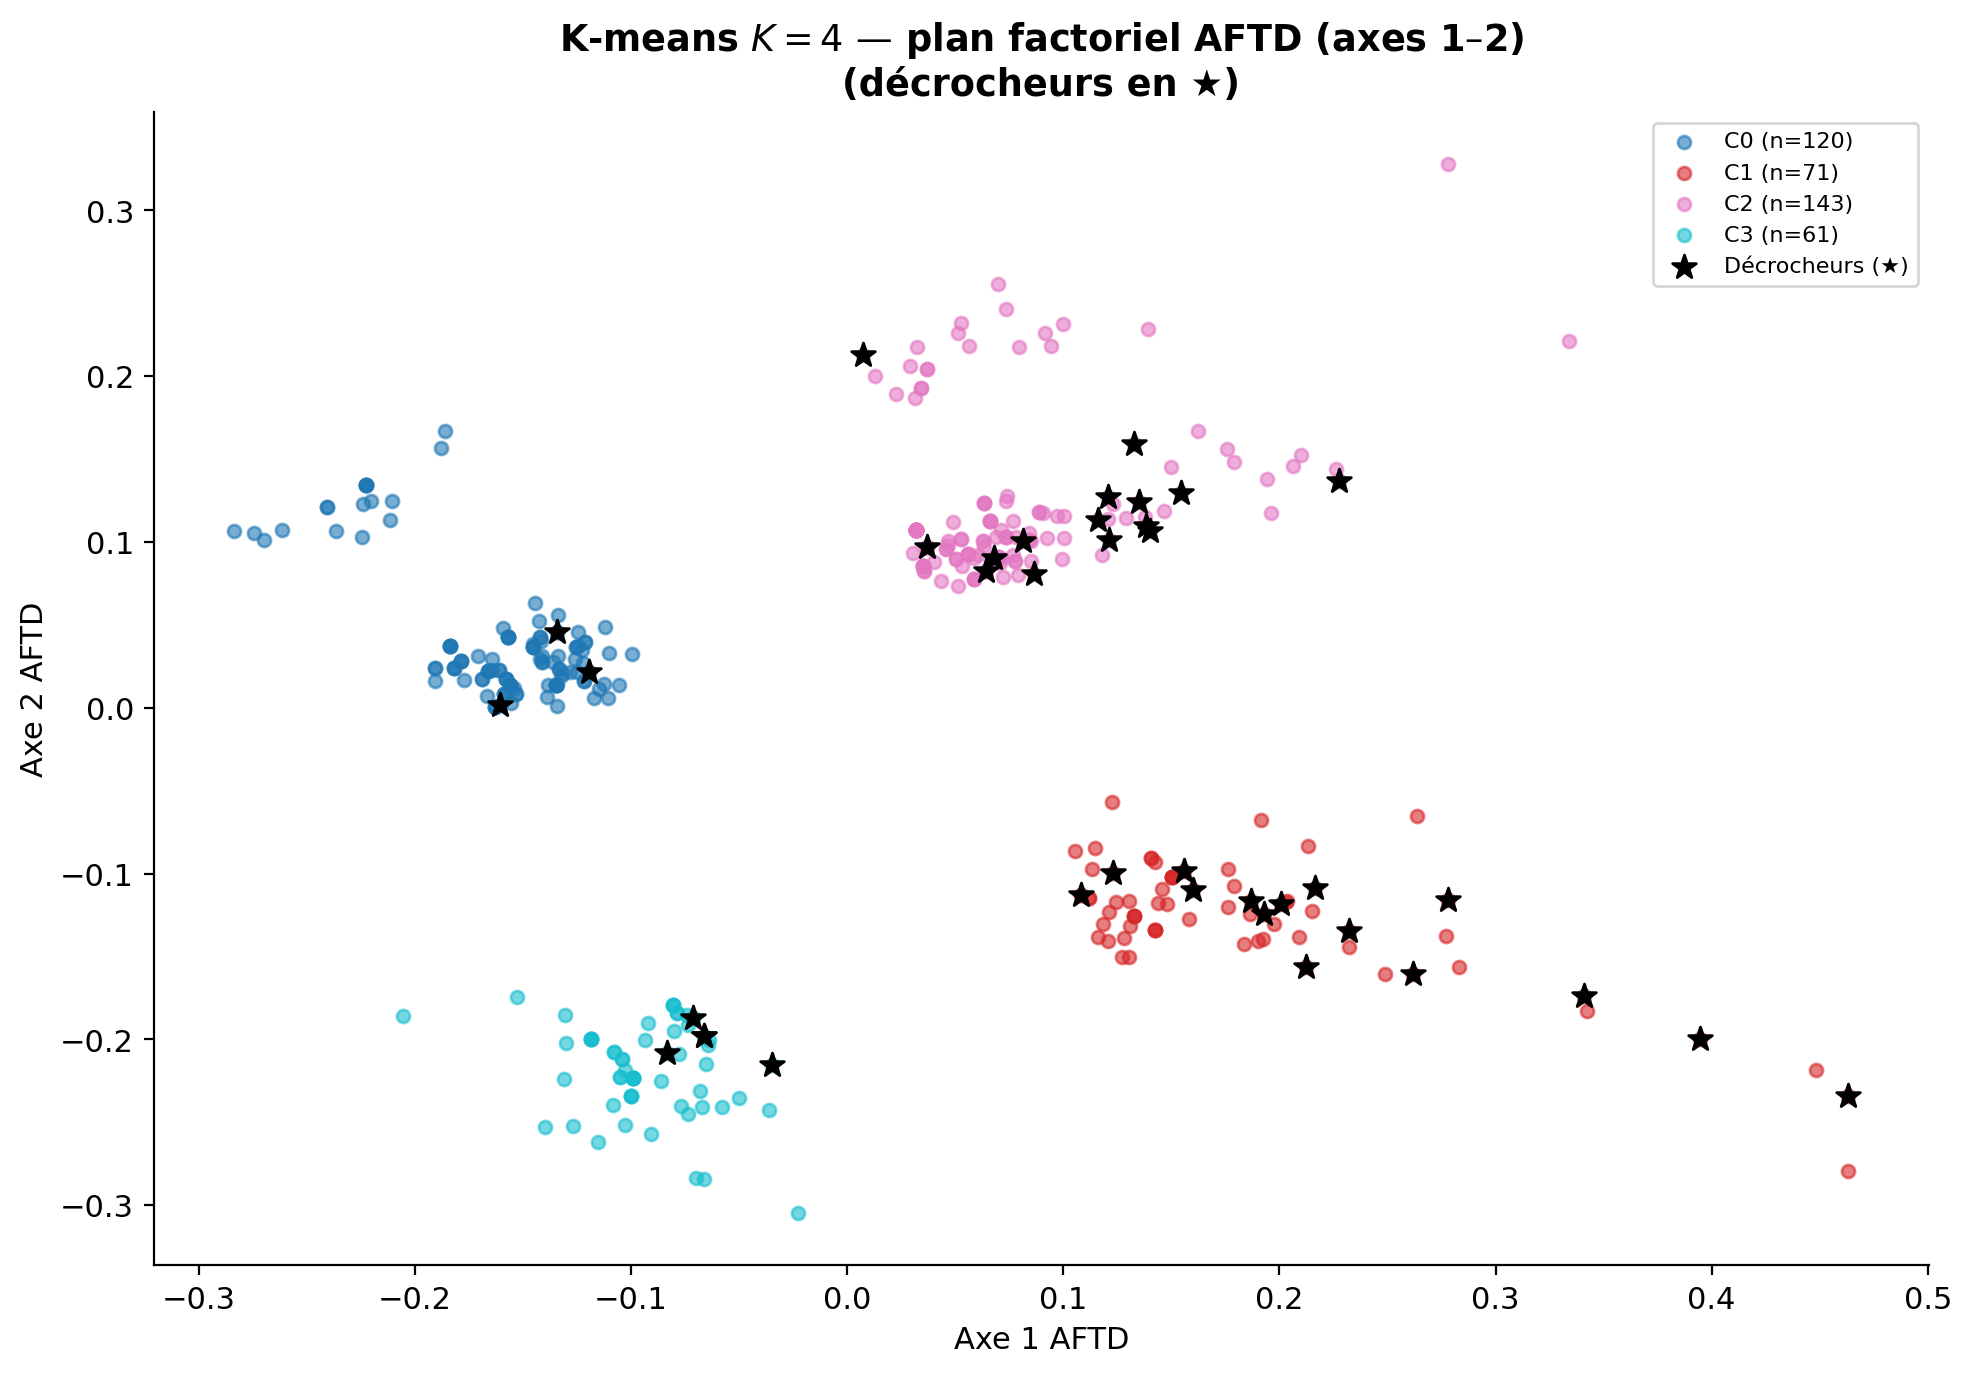
\includegraphics[width=0.95\columnwidth]{03_plan_factoriel_clusters.png}
\caption{Plan factoriel AFTD (axes 1--2) coloré par cluster $K$-means ($K=4$)~; décrocheurs en $\star$.}
\label{fig:plan_clusters}
\end{figure}

Le tableau~\ref{tab:profils} résume les taux de décrochage observés par cluster. La figure~\ref{fig:profils} présente les profils moyens normalisés sur les 8 variables de construction.

\begin{table}[h]
\caption{Taux de décrochage par cluster (K-means, $K=4$).}
\label{tab:profils}
\centering
\small
\begin{tabular}{lrr}
\toprule
Cluster & $n$ & Taux de décrochage \\
\midrule
C0 & 120 & 2{,}5\,\% \\
C1 & 71  & \textbf{21{,}1\,\%} \\
C2 & 143 & 10{,}5\,\% \\
C3 & 61  & 8{,}2\,\% \\
\bottomrule
\end{tabular}
\end{table}

\begin{figure}[h]
\centering
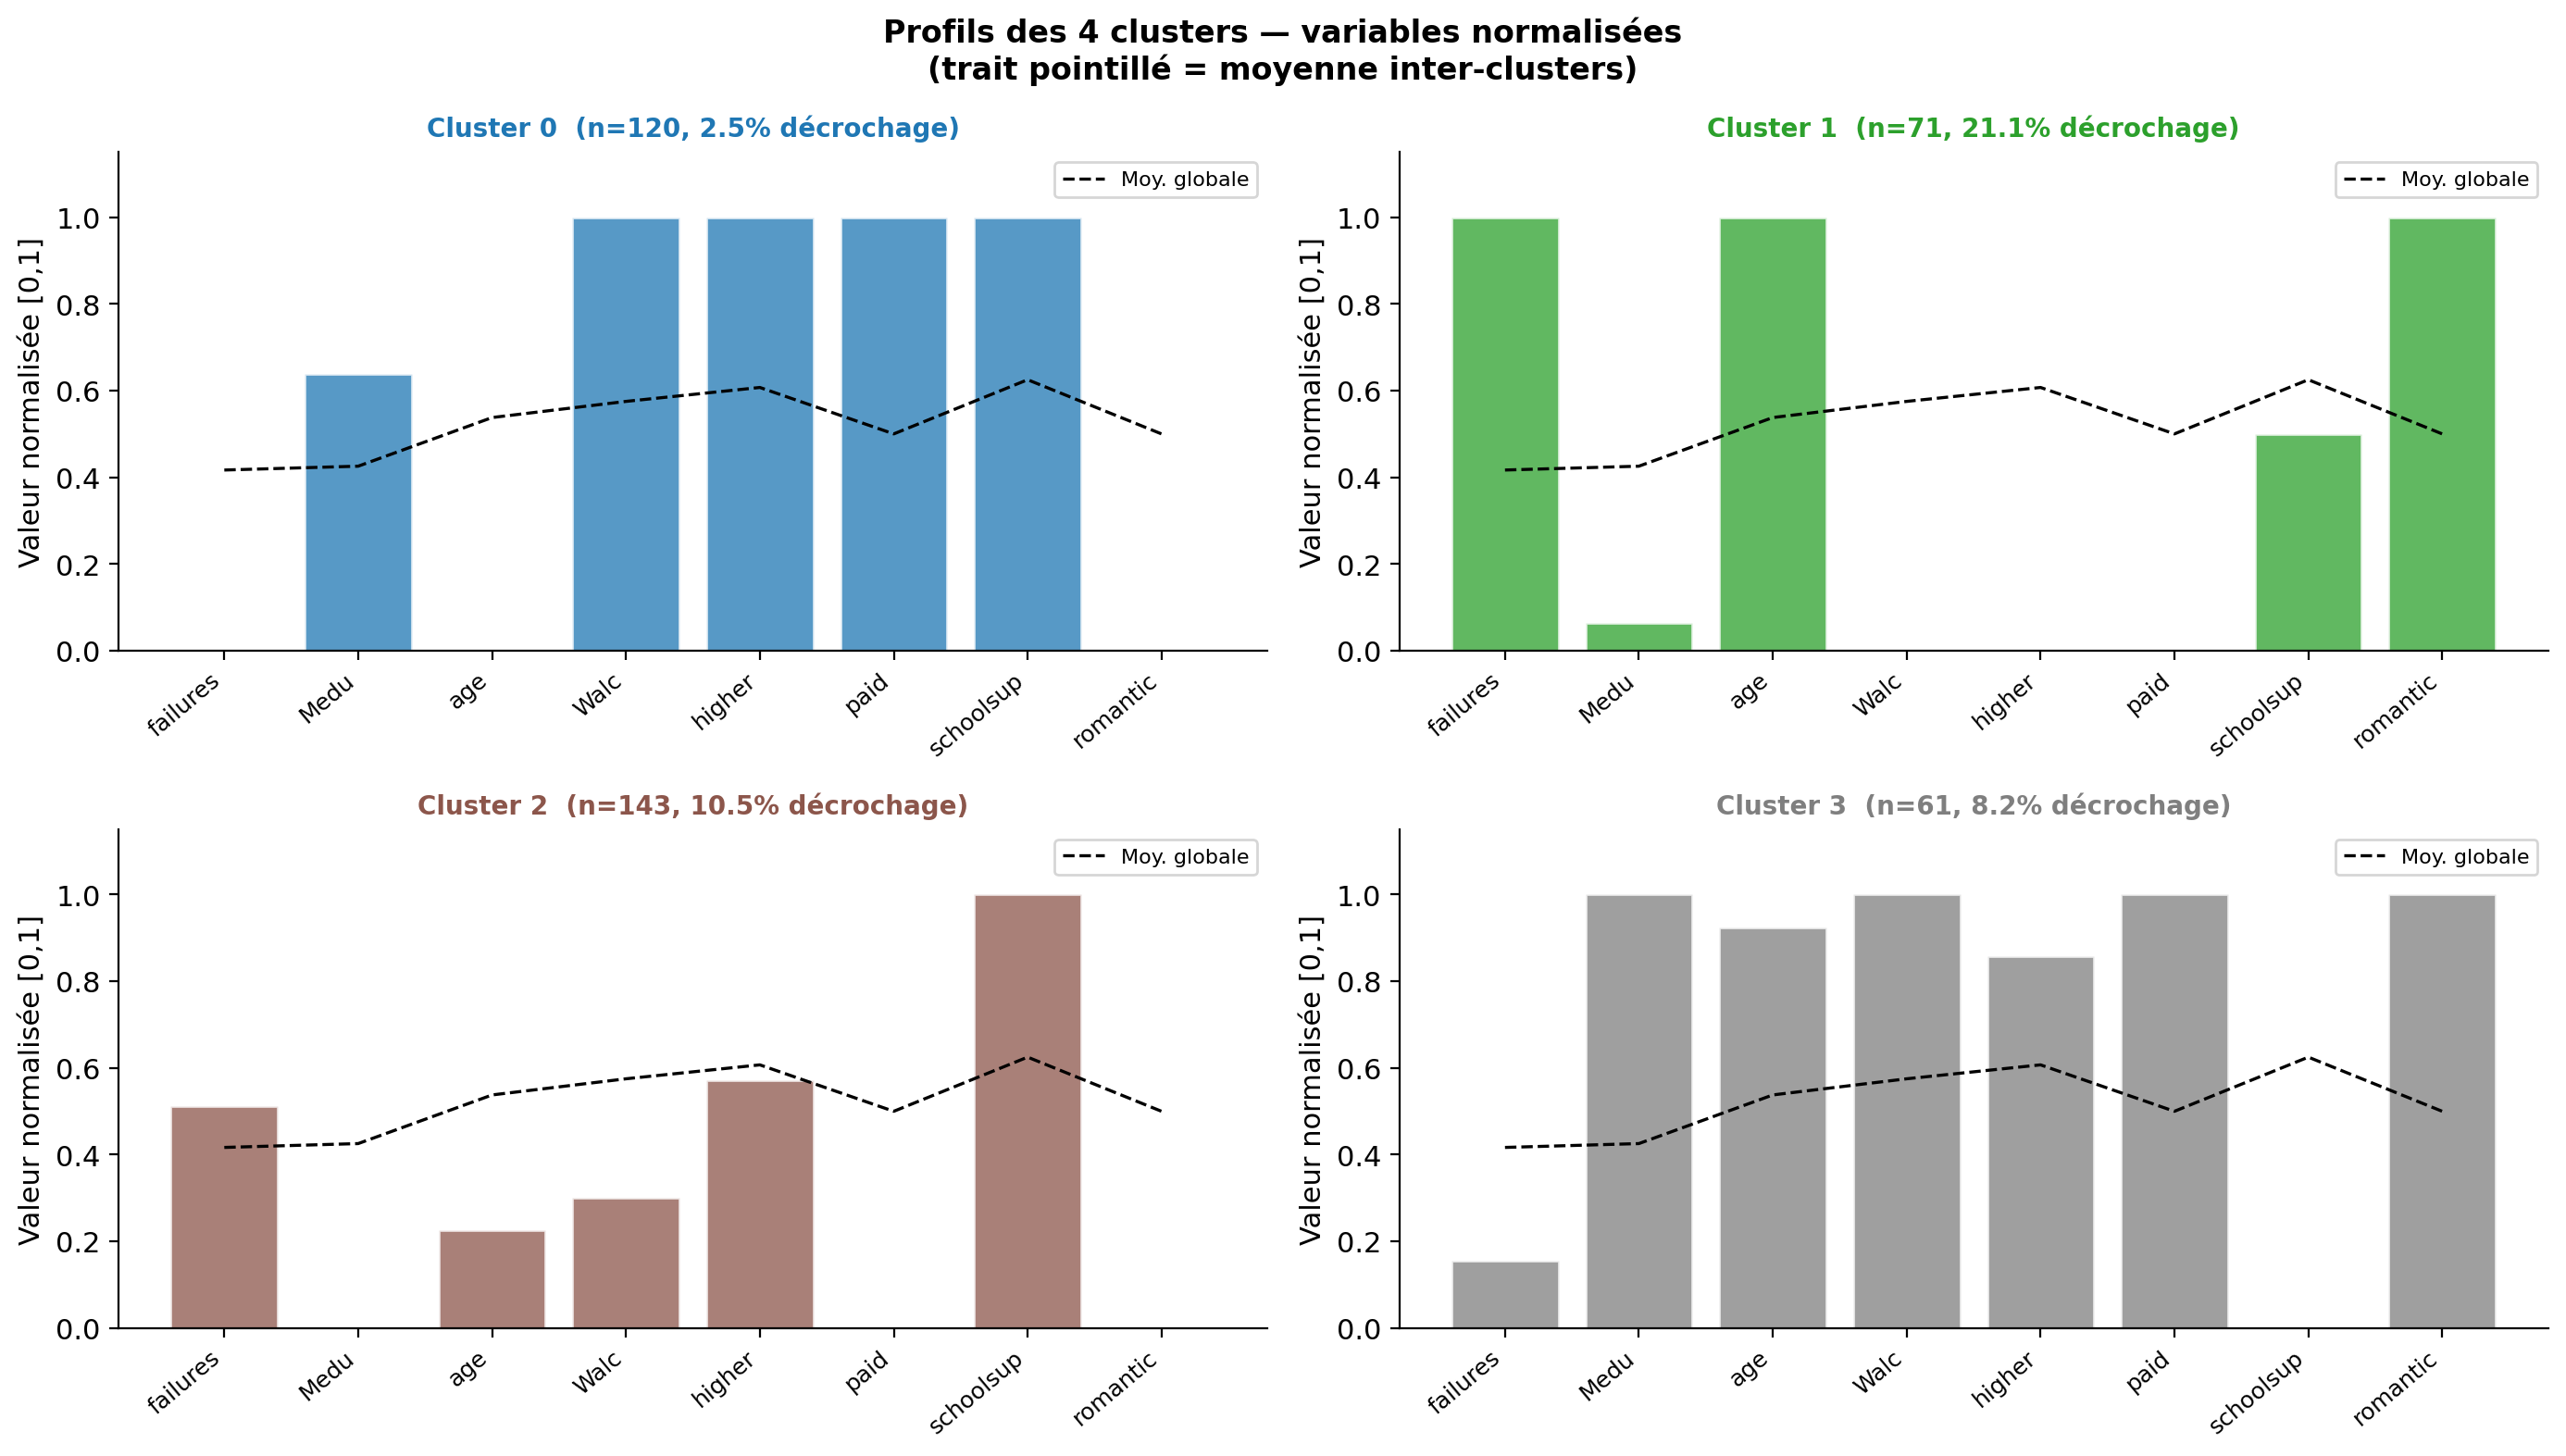
\includegraphics[width=0.95\columnwidth]{03_profils_clusters.png}
\caption{Profils des 4 clusters~: valeurs moyennes normalisées des 8 variables de construction.}
\label{fig:profils}
\end{figure}

\textit{C0} (n=120, 2,5\,\%)~: profil le plus protégé. Tous les élèves bénéficient de cours particuliers (\texttt{paid}=1) et se projettent vers les études supérieures (\texttt{higher}=1). Aucun n'est en relation amoureuse. Le niveau d'éducation maternel est élevé (\texttt{Medu}=2,88) et le nombre d'échecs antérieurs est faible (0,16).

\textit{C1} (n=71, 21,1\,\%)~: profil à risque dominant. Le taux d'échecs antérieurs est le plus élevé (\texttt{failures}=0,61), aucun élève ne suit de cours particuliers (\texttt{paid}=0), et tous sont en relation amoureuse (\texttt{romantic}=1). La projection vers les études supérieures est la plus faible des quatre clusters (86\,\%). Cet ensemble de facteurs cumulés explique un taux de décrochage 2,2 fois supérieur à la moyenne globale.

\textit{C2} (n=143, 10,5\,\%)~: profil intermédiaire et le plus peuplé. L'absence de cours particuliers (\texttt{paid}=0) distingue ce cluster de C0, mais l'absence de relation amoureuse (\texttt{romantic}=0) le distingue de C1. Le taux d'échecs antérieurs est modéré (0,39).

\textit{C3} (n=61, 8,2\,\%)~: profil protégé mais non maximal. Le niveau d'éducation maternel est le plus élevé des quatre clusters (\texttt{Medu}=3,05) et les élèves bénéficient de cours particuliers (\texttt{paid}=1). La présence de relations amoureuses (\texttt{romantic}=1) différencie ce groupe de C0, sans pour autant se traduire par un taux de décrochage aussi bas.

\textit{Note sur la consommation d'alcool.} Bien que \texttt{Walc} soit sélectionnée comme variable discriminante lors des tests préliminaires, le cluster à risque C1 présente la consommation d'alcool le weekend la plus faible des quatre profils (\texttt{Walc}=2,18 contre 2,38 pour C0 et C3), ce qui va à l'encontre de l'intuition et suggère que cette variable intervient davantage comme signal de différenciation inter-clusters que comme facteur de risque direct.

La contribution des variables aux axes factoriels (figure~\ref{fig:ann_contrib}, annexe~\ref{ann:contrib}) révèle que \texttt{paid} structure majoritairement l'axe 1 (54,8\,\% de contribution), \texttt{romantic} domine l'axe 2 (73,1\,\%), et \texttt{Walc} et \texttt{schoolsup} sont les variables les plus liées à l'axe 3 (38,2\,\% et 22,5\,\% respectivement).

\section{Validation et apprentissage supervisé}
\label{sec:validation}

\subsection{Lien cluster/décrochage}

Un test du $\chi^2$ d'indépendance~\cite[Ch.\,12, \S\,12.1]{polySY02} est appliqué entre la partition en 4 clusters et la variable \texttt{decrocheur}. L'association est très hautement significative ($\chi^2 = 18{,}1$, $p < 0{,}001$, ddl\,=\,3). Le V de Cramér vaut 0,214~: l'intensité de l'association est modérée, ce qui indique que la structure non supervisée capture un signal réel et non un artefact.

\subsection{Classifieurs supervisés}

Quatre classifieurs~\cite[Ch.\,10--12]{polySY09} sont entraînés sur les 8 variables socio-comportementales (sans G1, G2, G3) pour prédire \texttt{decrocheur}~: Analyse Discriminante Linéaire (LDA), régression logistique, arbre CART (critère de Gini) et gradient boosting (LightGBM). Le fort déséquilibre de classes (1~:~9) est corrigé en pondérant les erreurs sur la classe minoritaire de façon inversement proportionnelle à ses effectifs.

Le risque est estimé par quatre méthodes~\cite[Ch.\,13]{polySY09}~: resubstitution (biaisée, borne inférieure), holdout stratifié 75/25, validation croisée 5-fold et bootstrap 0,632. Le tableau~\ref{tab:classifieurs} présente les résultats.

\begin{table}[h]
\caption{Taux d'erreur estimés et AUC-ROC en validation croisée 5-fold. La resubstitution est biaisée vers le bas~; CV-5 et Bootstrap 0,632 sont les estimateurs de référence~\cite[Ch.\,13]{polySY09}.}
\label{tab:classifieurs}
\centering
\footnotesize
\begin{tabular}{lrrrrc}
\toprule
 & Resub. & Holdout & CV-5 & Boot.632 & AUC \\
\midrule
LDA      & 0,099 & 0,101 & 0,109 & 0,106 & 0,746 \\
LogReg   & 0,243 & 0,242 & 0,258 & 0,259 & \textbf{0,757} \\
CART     & 0,243 & 0,263 & 0,273 & 0,270 & 0,632 \\
LightGBM & 0,149 & 0,162 & 0,200 & 0,177 & 0,702 \\
\bottomrule
\end{tabular}
\end{table}

La LDA obtient le taux d'erreur CV le plus bas (10,9\,\%), mais son faible taux d'erreur s'explique en partie par une tendance à classer par défaut les individus dans la classe majoritaire (non-décrocheurs, 90,4\,\%). L'AUC-ROC, moins sensible à ce biais, est plus pertinente~: la régression logistique obtient la valeur la plus élevée (0,757 en CV-5) et est retenue comme classifieur de référence.

\subsection{Règle de Neyman-Pearson}

Dans un contexte d'alerte précoce, le coût d'un décrocheur non détecté est supérieur à celui d'une fausse alarme. La règle de Neyman-Pearson~\cite[Ch.\,9]{polySY09} est appliquée sur la régression logistique~: le rappel (taux de vrais positifs) est maximisé sous la contrainte $\text{FPR} \leq \alpha^* = 0{,}20$. Cette règle améliore la détection par rapport au seuil de décision par défaut, au prix d'une augmentation des fausses alarmes. La courbe ROC et les matrices de confusion associées sont reportées en annexe~\ref{ann:roc} (figure~\ref{fig:ann_roc}).

\section{Conclusion}

\subsection{Synthèse du clustering}

L'AFTD et le clustering identifient une structure en 4 profils robuste et stable (ARI$\approx$1). La partition est statistiquement significative~: les variables \texttt{paid}, \texttt{higher} et \texttt{failures} sont les plus discriminantes entre profils selon les tests post-hoc avec correction de Bonferroni. Le profil C1 concentre 21,1\,\% de décrocheurs (contre 9,6\,\% en moyenne)~; à l'opposé, C0 présente un taux de 2,5\,\%. Ces résultats montrent que des variables socio-comportementales disponibles en début d'année permettent de structurer la population en profils dont les niveaux de risque diffèrent significativement.

La limite principale de cette étape réside dans la taille de l'échantillon~: 395 élèves issus d'une seule cohorte, avec 38 décrocheurs seulement. Les centroïdes identifiés sont spécifiques à cette cohorte et leur généralisation à d'autres établissements reste à vérifier. Par ailleurs, l'appartenance au cluster C1 caractérise un profil de vulnérabilité, mais ne constitue pas une prédiction individuelle du décrochage.

\subsection{Synthèse de la validation supervisée}

Le lien entre la partition non supervisée et le décrochage est statistiquement établi ($\chi^2 = 18{,}1$, $p < 0{,}001$, $V = 0{,}214$)~: la structure des profils capture bien un signal réel dans les données. Du côté de la prédiction individuelle, l'AUC-ROC de la régression logistique atteint 0,757 en validation croisée, ce qui représente une discrimination au-delà de l'aléatoire. Cependant, la prédiction individuelle reste difficile en raison du fort déséquilibre des classes~; la règle de Neyman-Pearson permet d'augmenter le rappel sous contrainte de faux positifs, ce qui est plus adapté à un dispositif d'alerte précoce (annexe~\ref{ann:roc}).

La variable \texttt{failures} ressort comme le signal le plus discriminant dans toutes les approches menées. Les variables \texttt{Medu} et \texttt{age} occupent des rangs élevés dans les importances des différents modèles. En revanche, la place de \texttt{Walc} dans les classifieurs supervisés diffère de son rôle dans la construction des profils~: sa contribution reste modeste à l'échelle individuelle, ce qui est cohérent avec la tendance contre-intuitive observée dans les profils (C1 présente une consommation d'alcool plus faible que C0).

Les données déclaratives utilisées introduisent un risque de biais de désirabilité sociale, et l'absence de G2 dans le vecteur de variables limite l'exploitation de l'information temporelle disponible. Ces deux points constituent des pistes d'amélioration pour de futurs travaux.

\clearpage
\onecolumn
\appendix

\section{Comparaisons univariées décrocheurs / non-décrocheurs}
\label{ann:discriminants}

Boxplots (variables numériques) et barres de proportions (variables catégorielles) pour les variables dont la $p$-valeur est inférieure à 0,10 lors de l'analyse préliminaire (mathématiques, $n=38$ décrocheurs).

\begin{figure}[H]
\centering
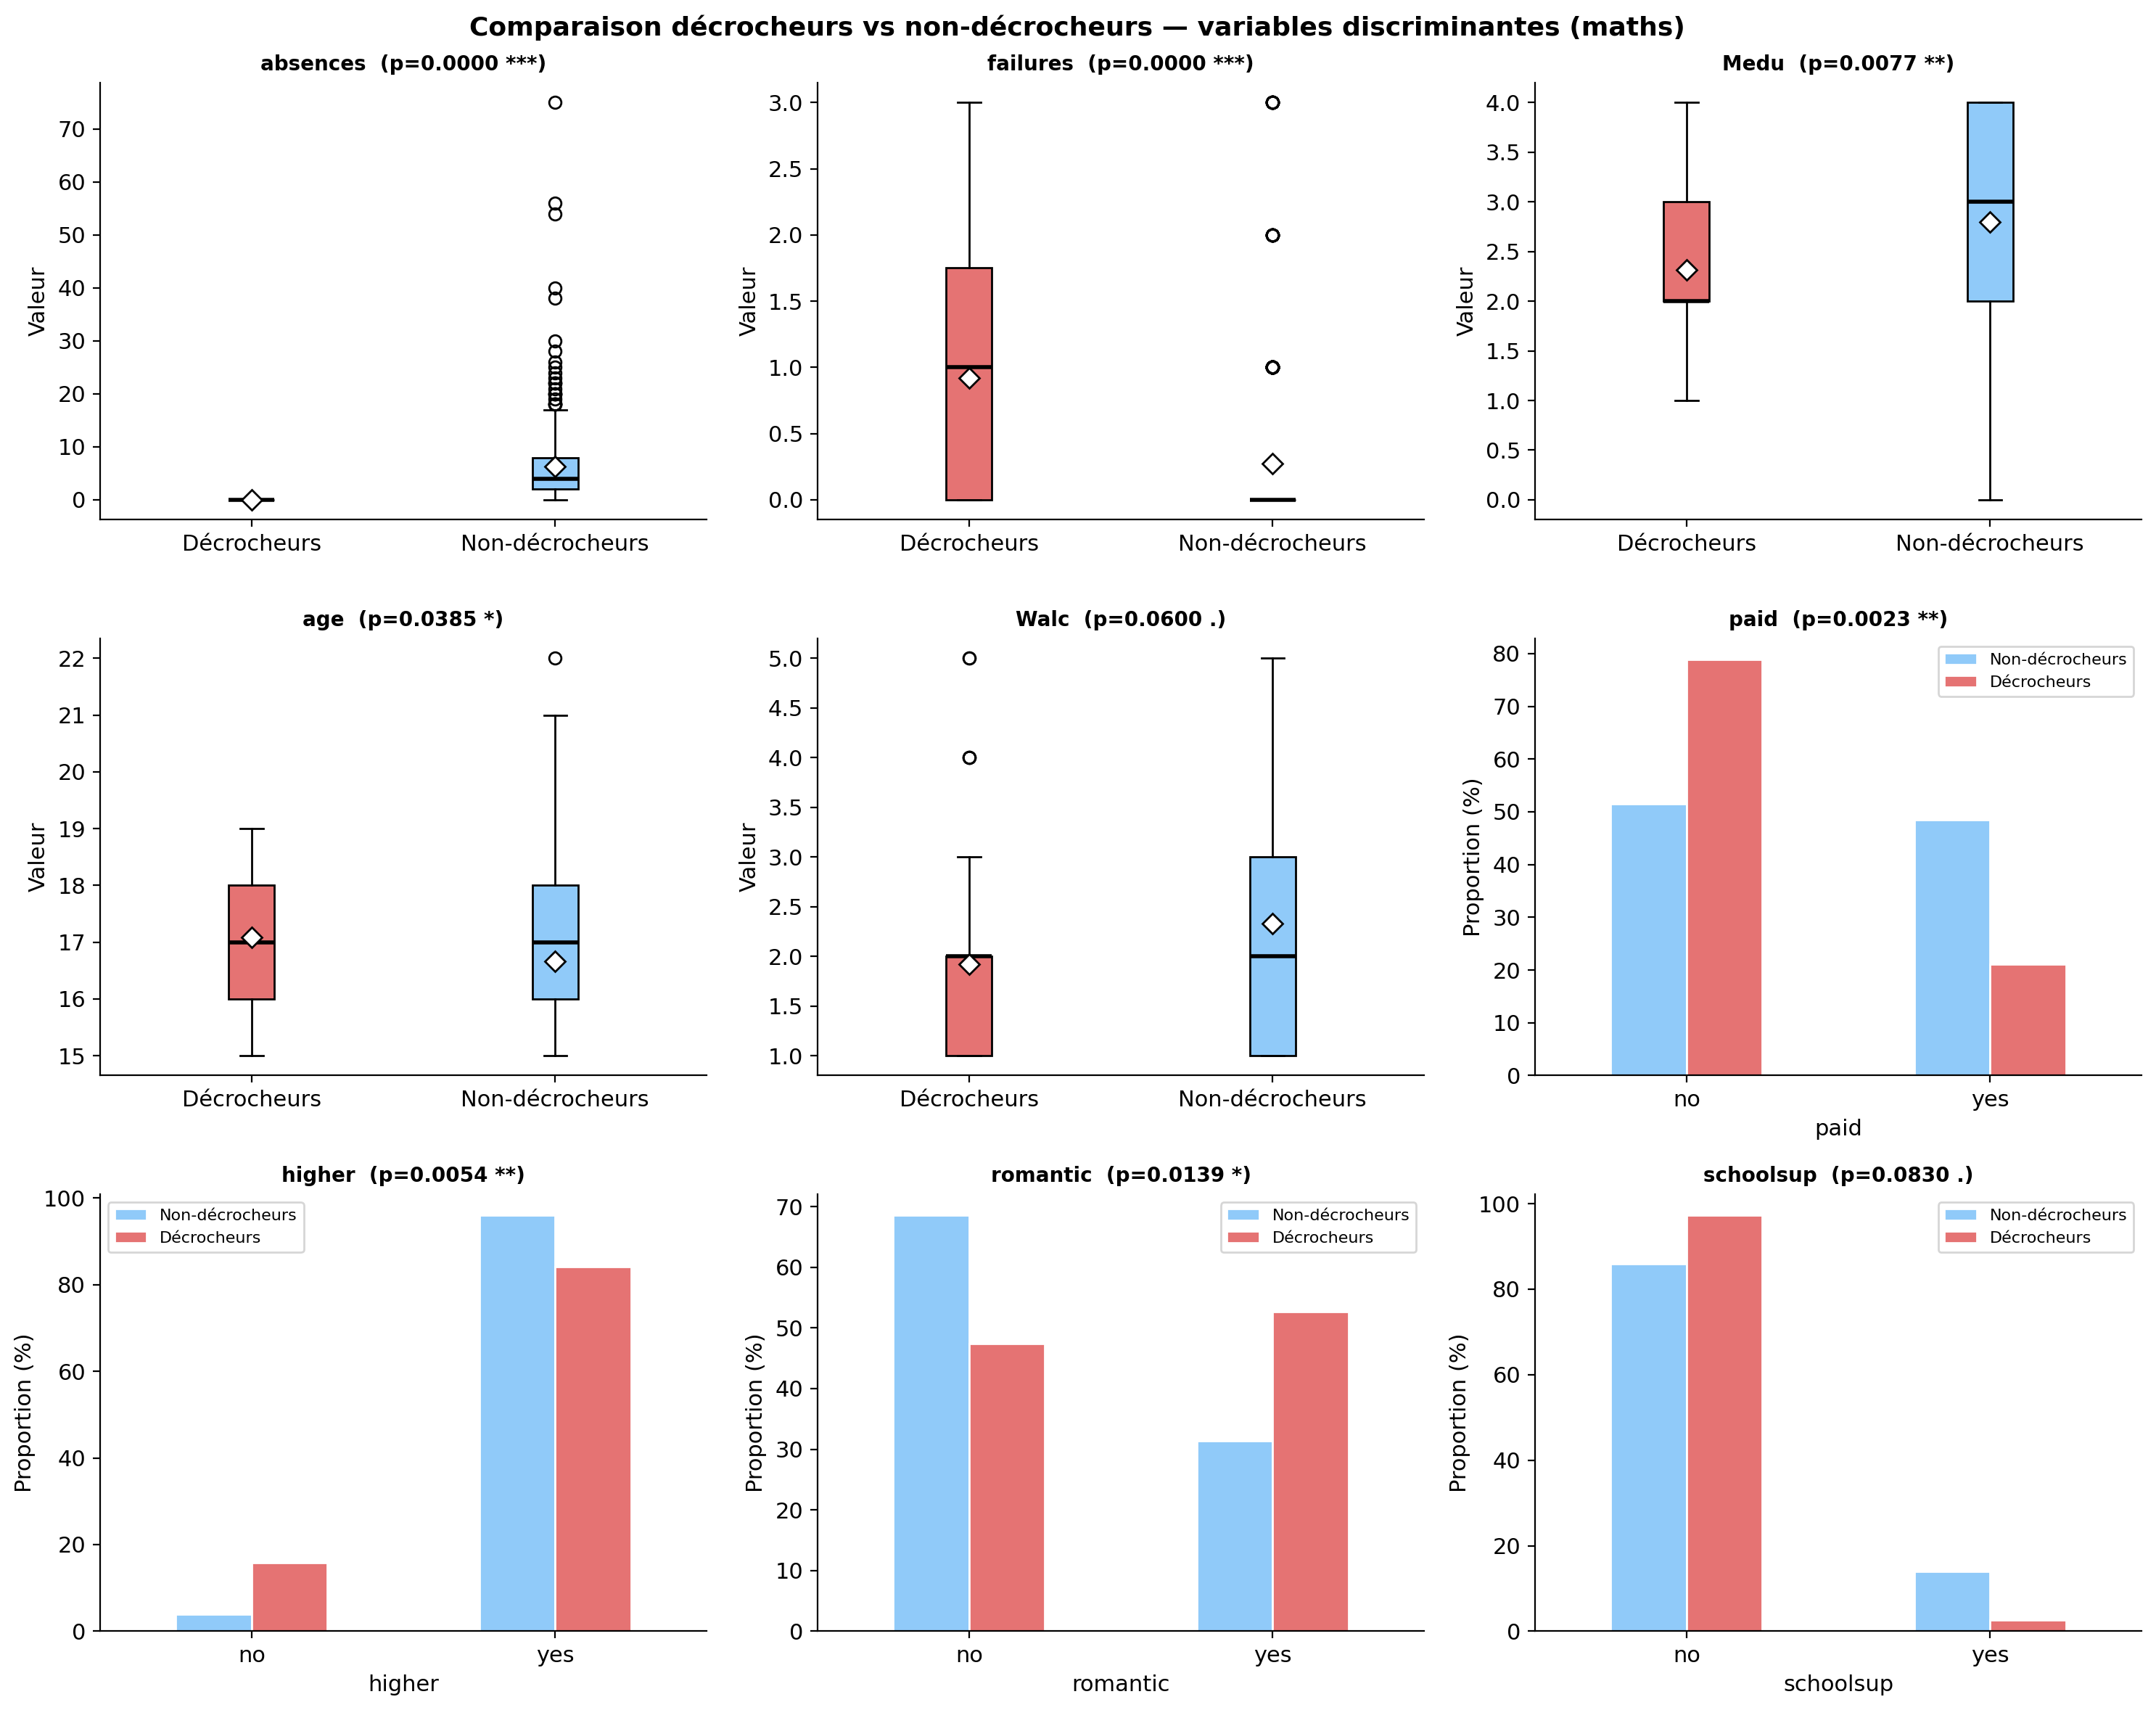
\includegraphics[width=0.92\textwidth]{00_discriminants.png}
\caption{Variables discriminantes~: comparaison décrocheurs vs non-décrocheurs ($\alpha = 0{,}10$).}
\label{fig:ann_discriminants}
\end{figure}
\clearpage

\section{Dendrogramme CAH-Ward et sélection de $K$}
\label{ann:cah}

Dendrogramme tronqué (15 dernières fusions) et sauts d'inertie Ward sur les coordonnées AFTD 3D. Le saut maximal pour $K \geq 3$ suggère $K=4$, en cohérence avec le score de silhouette du $K$-means.

\begin{figure}[H]
\centering
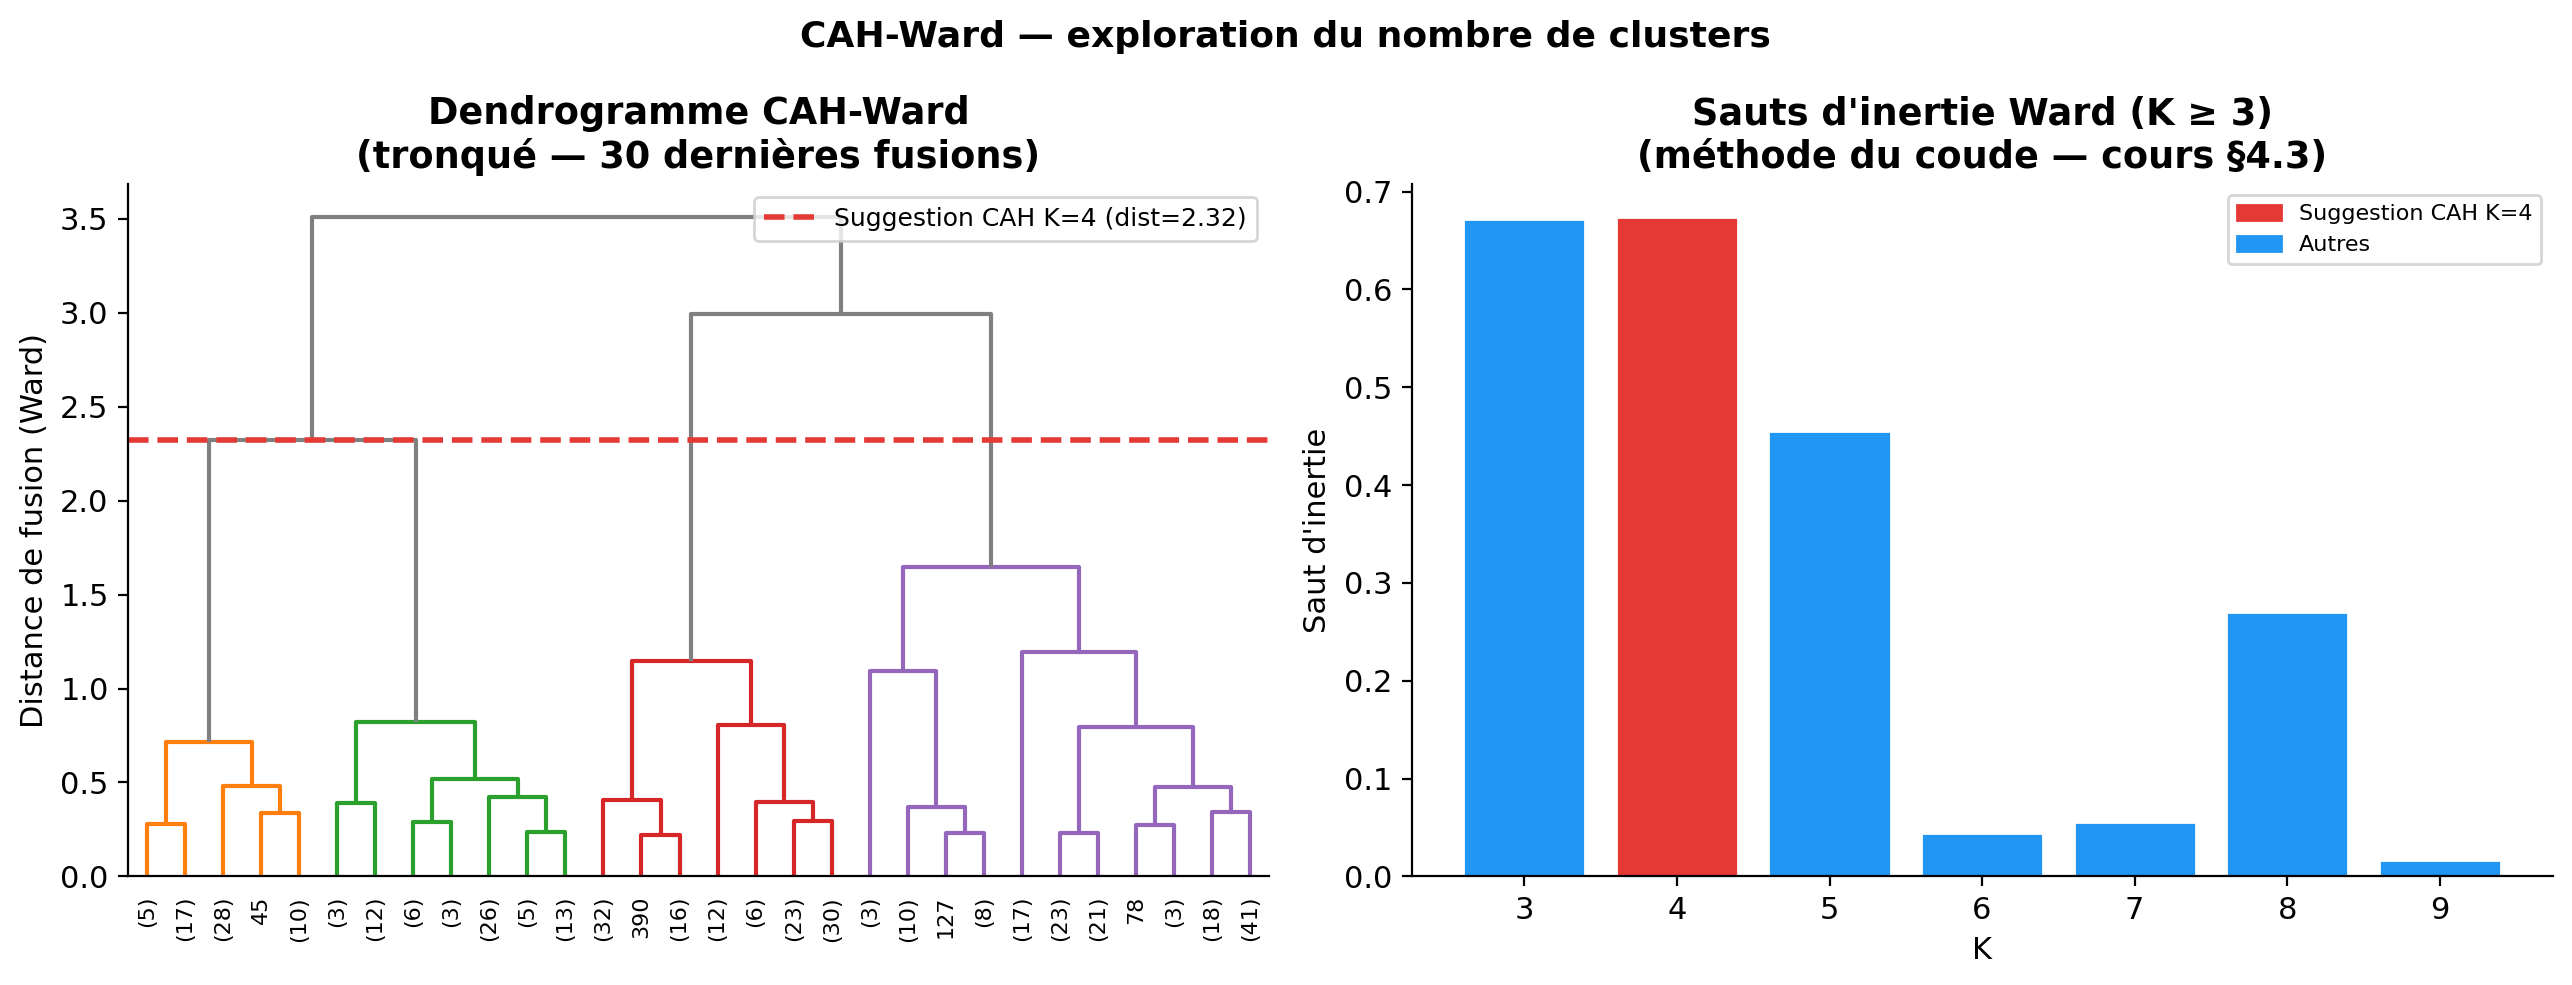
\includegraphics[width=0.92\textwidth]{03_cah_dendrogramme.png}
\caption{CAH-Ward~: dendrogramme et exploration du nombre de clusters.}
\label{fig:ann_cah}
\end{figure}

\section{Sélection de $K$ par coude et silhouette ($K$-means)}
\label{ann:coude_sil}

Courbes d'inertie intra-classe et de silhouette moyenne sur $K \in [3, 10]$. Le coude suggère $K=5$~; la silhouette maximale retient $K=4$.

\begin{figure}[H]
\centering
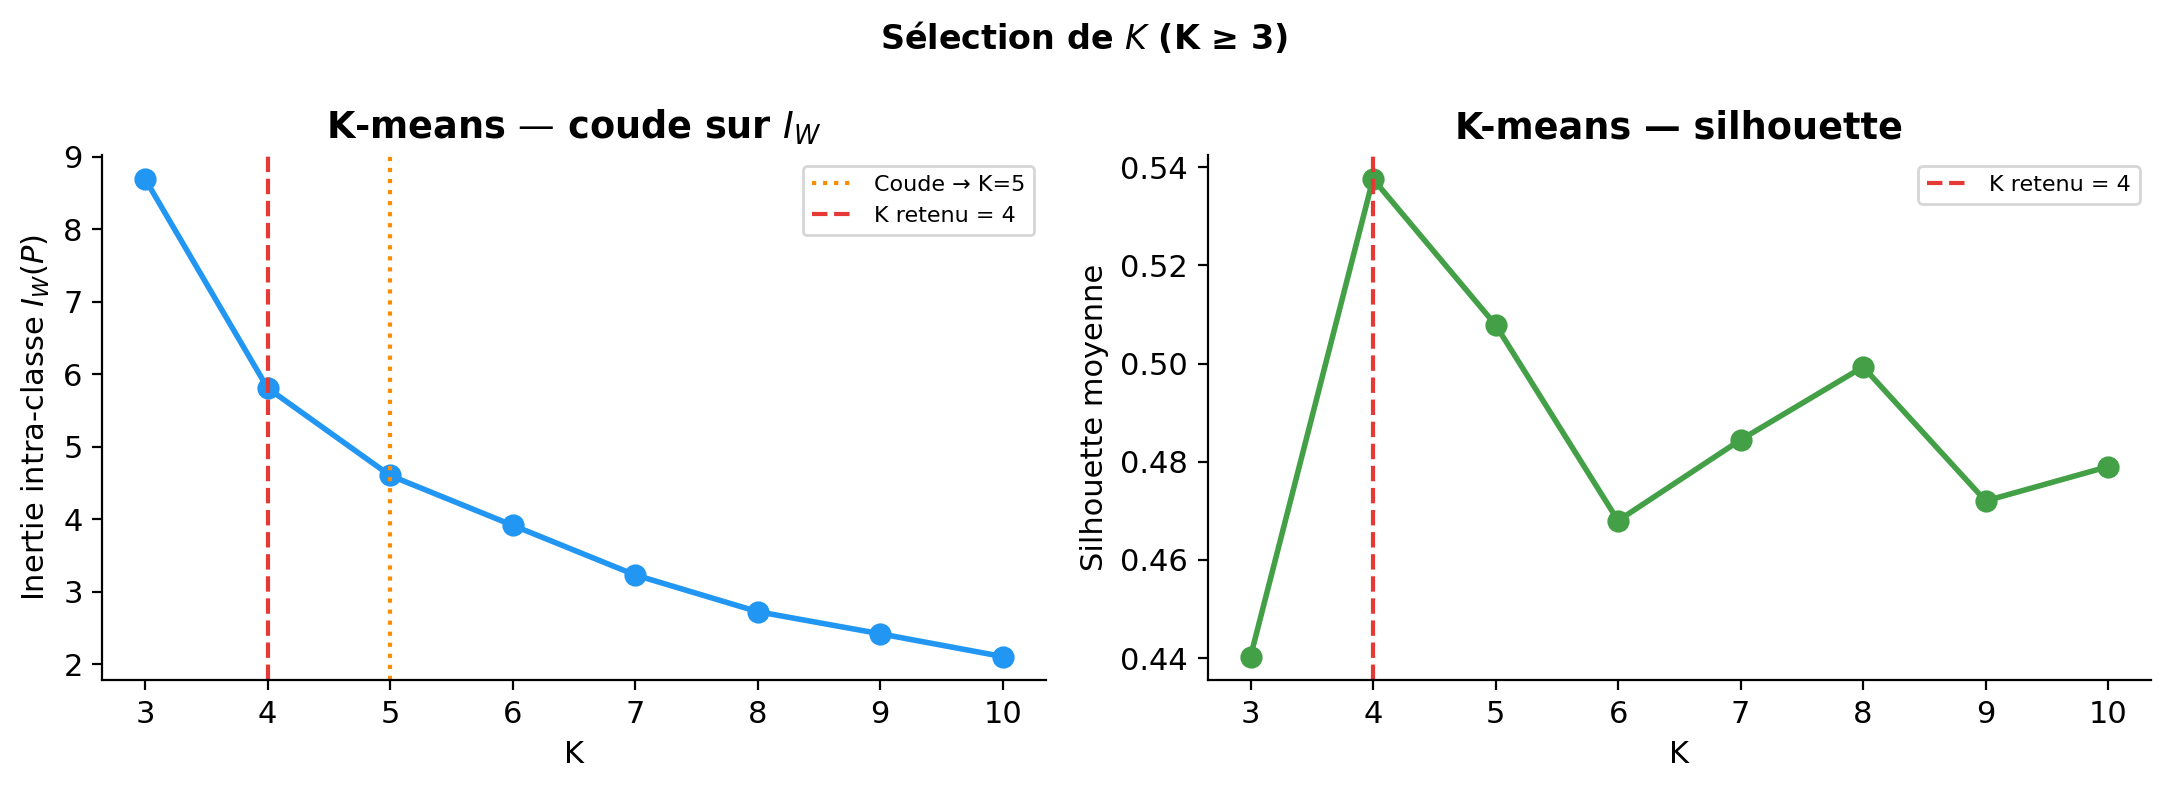
\includegraphics[width=0.88\textwidth]{03_kmeans_coude_silhouette.png}
\caption{$K$-means~: méthode du coude et score de silhouette.}
\label{fig:ann_coude_sil}
\end{figure}
\clearpage

\section{Contributions des variables aux axes AFTD}
\label{ann:contrib}

Contributions normalisées (cos² de la corrélation de Pearson) des 8 variables actives aux 3 axes factoriels retenus.

\begin{figure}[H]
\centering
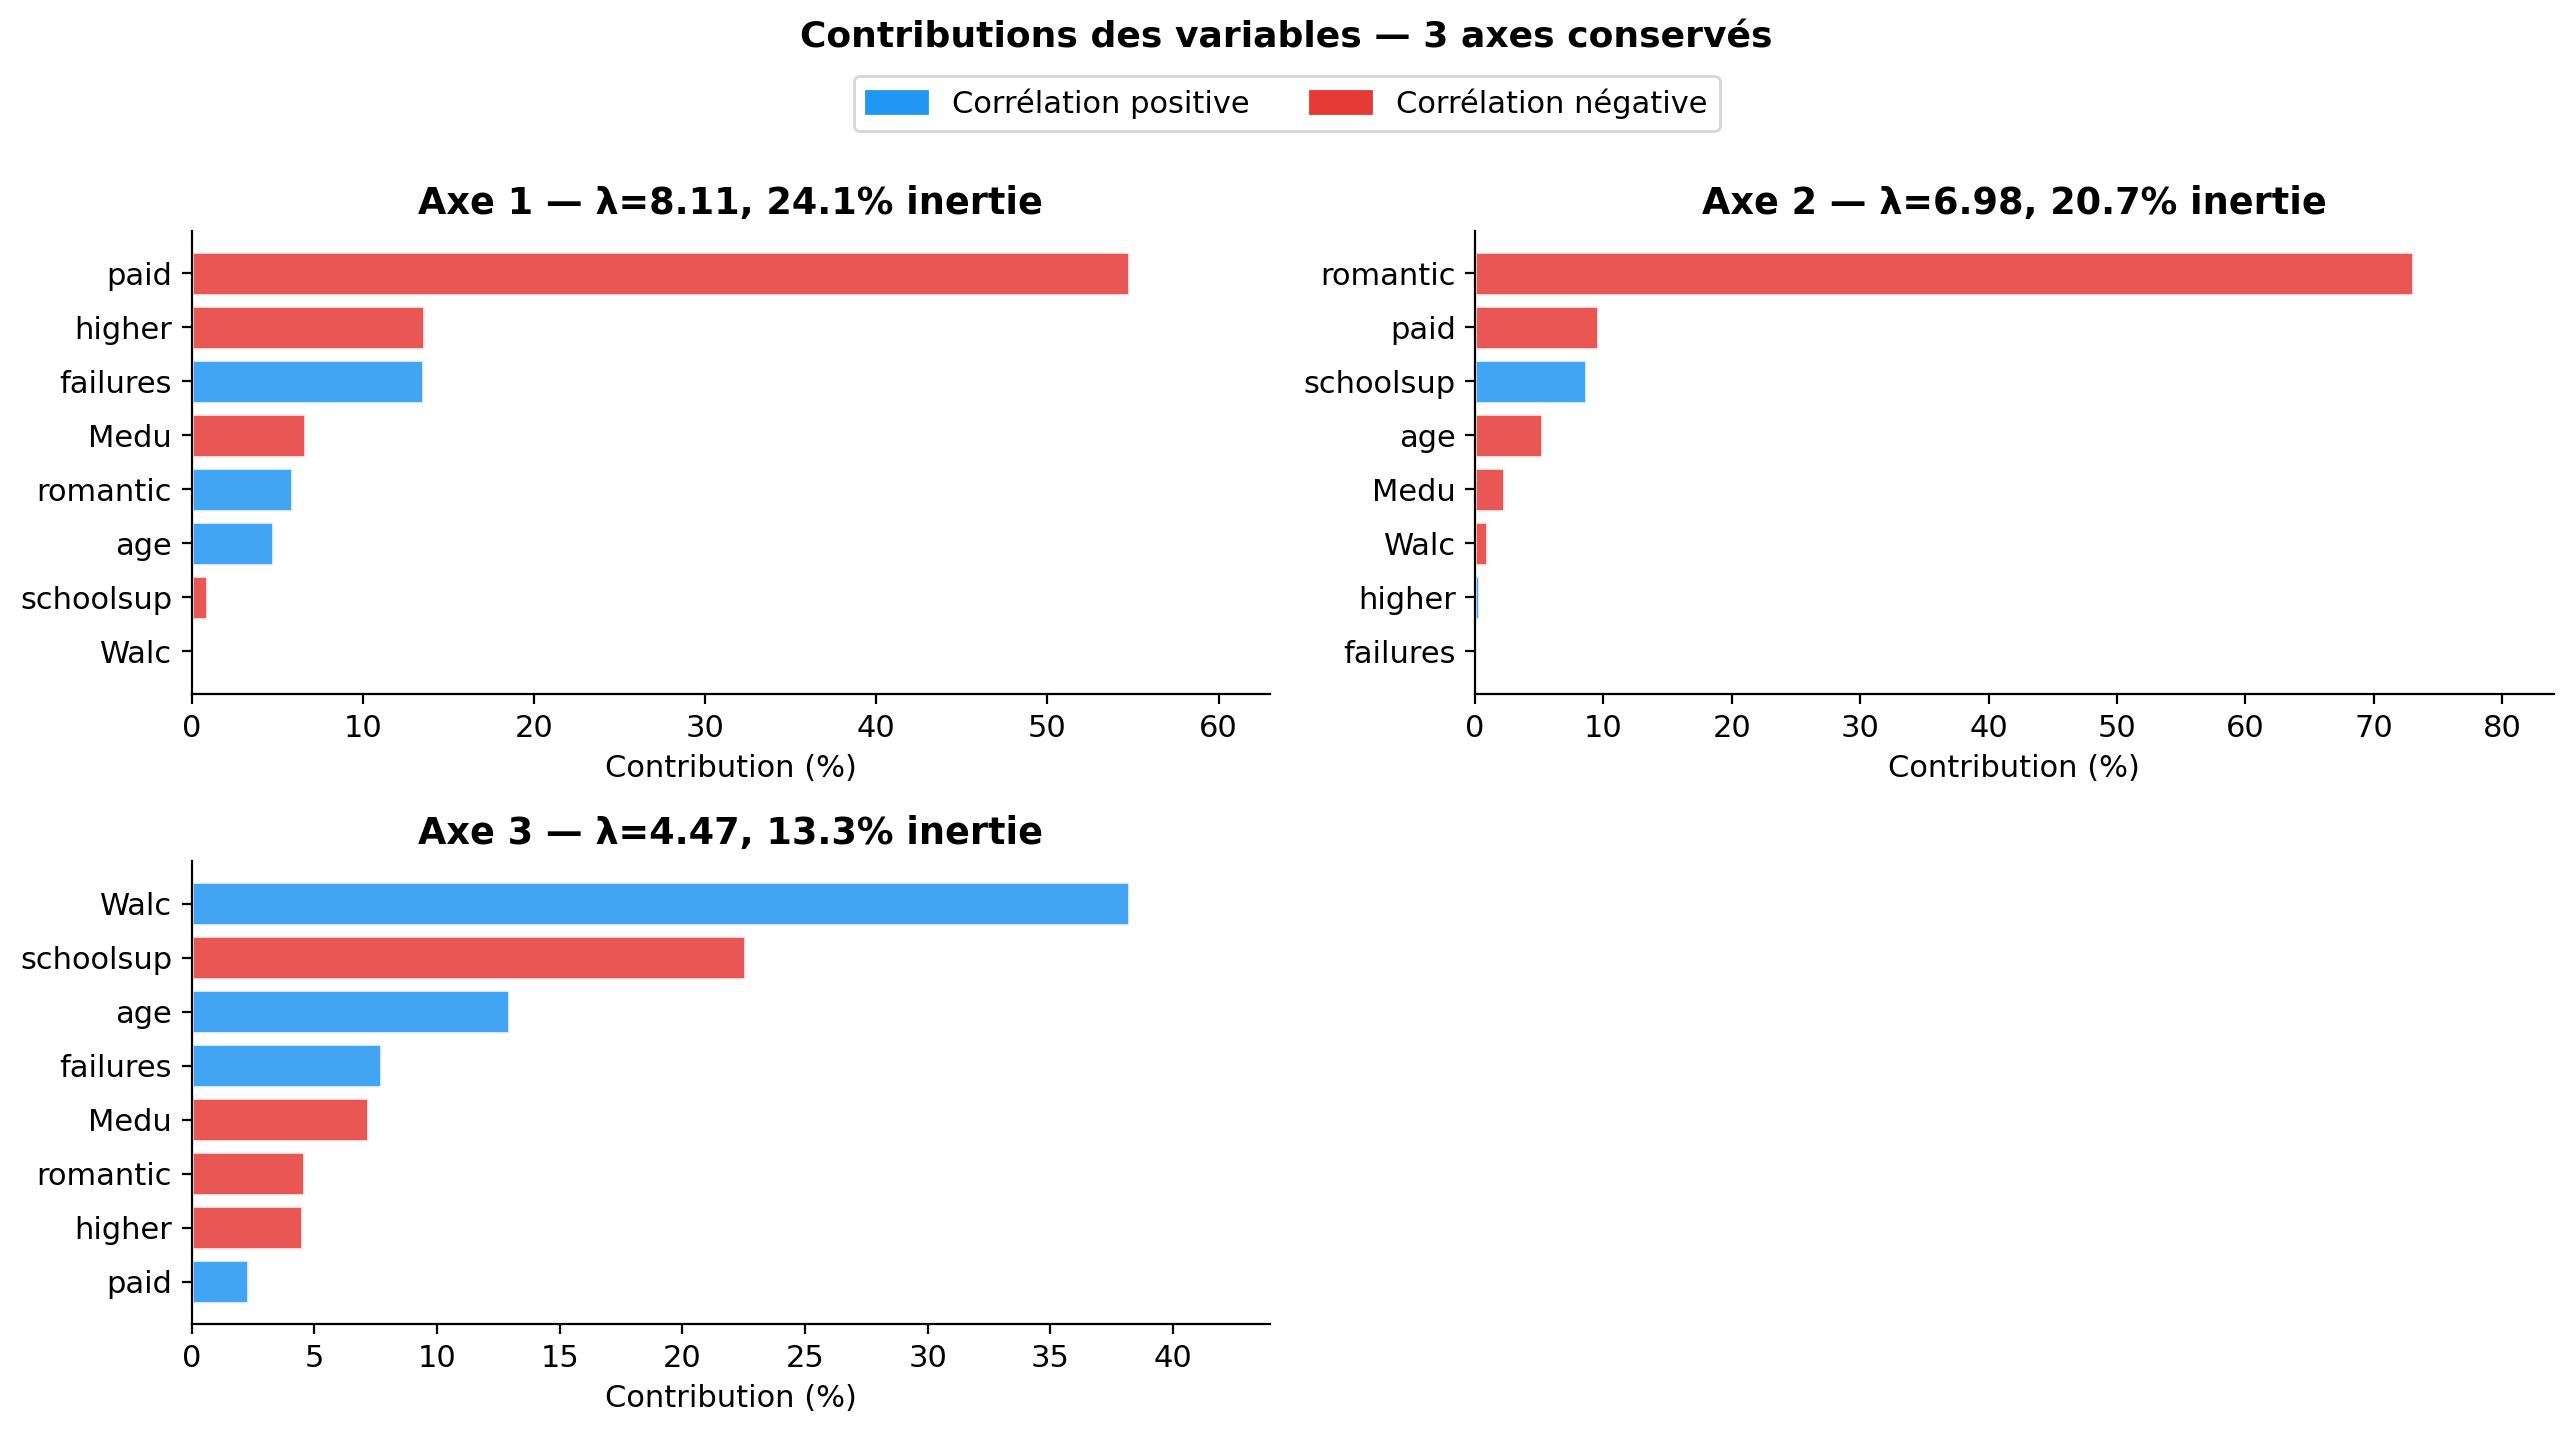
\includegraphics[width=0.92\textwidth]{03_contributions_variables.png}
\caption{Contributions des variables aux 3 axes AFTD conservés.}
\label{fig:ann_contrib}
\end{figure}

\section{Courbe ROC et règle de Neyman-Pearson}
\label{ann:roc}

Courbe ROC de la régression logistique (AUC CV-5 = 0,757) et comparaison des matrices de confusion au seuil 0,5 vs seuil optimal sous contrainte FPR~$\leq 0{,}20$.

\begin{figure}[H]
\centering
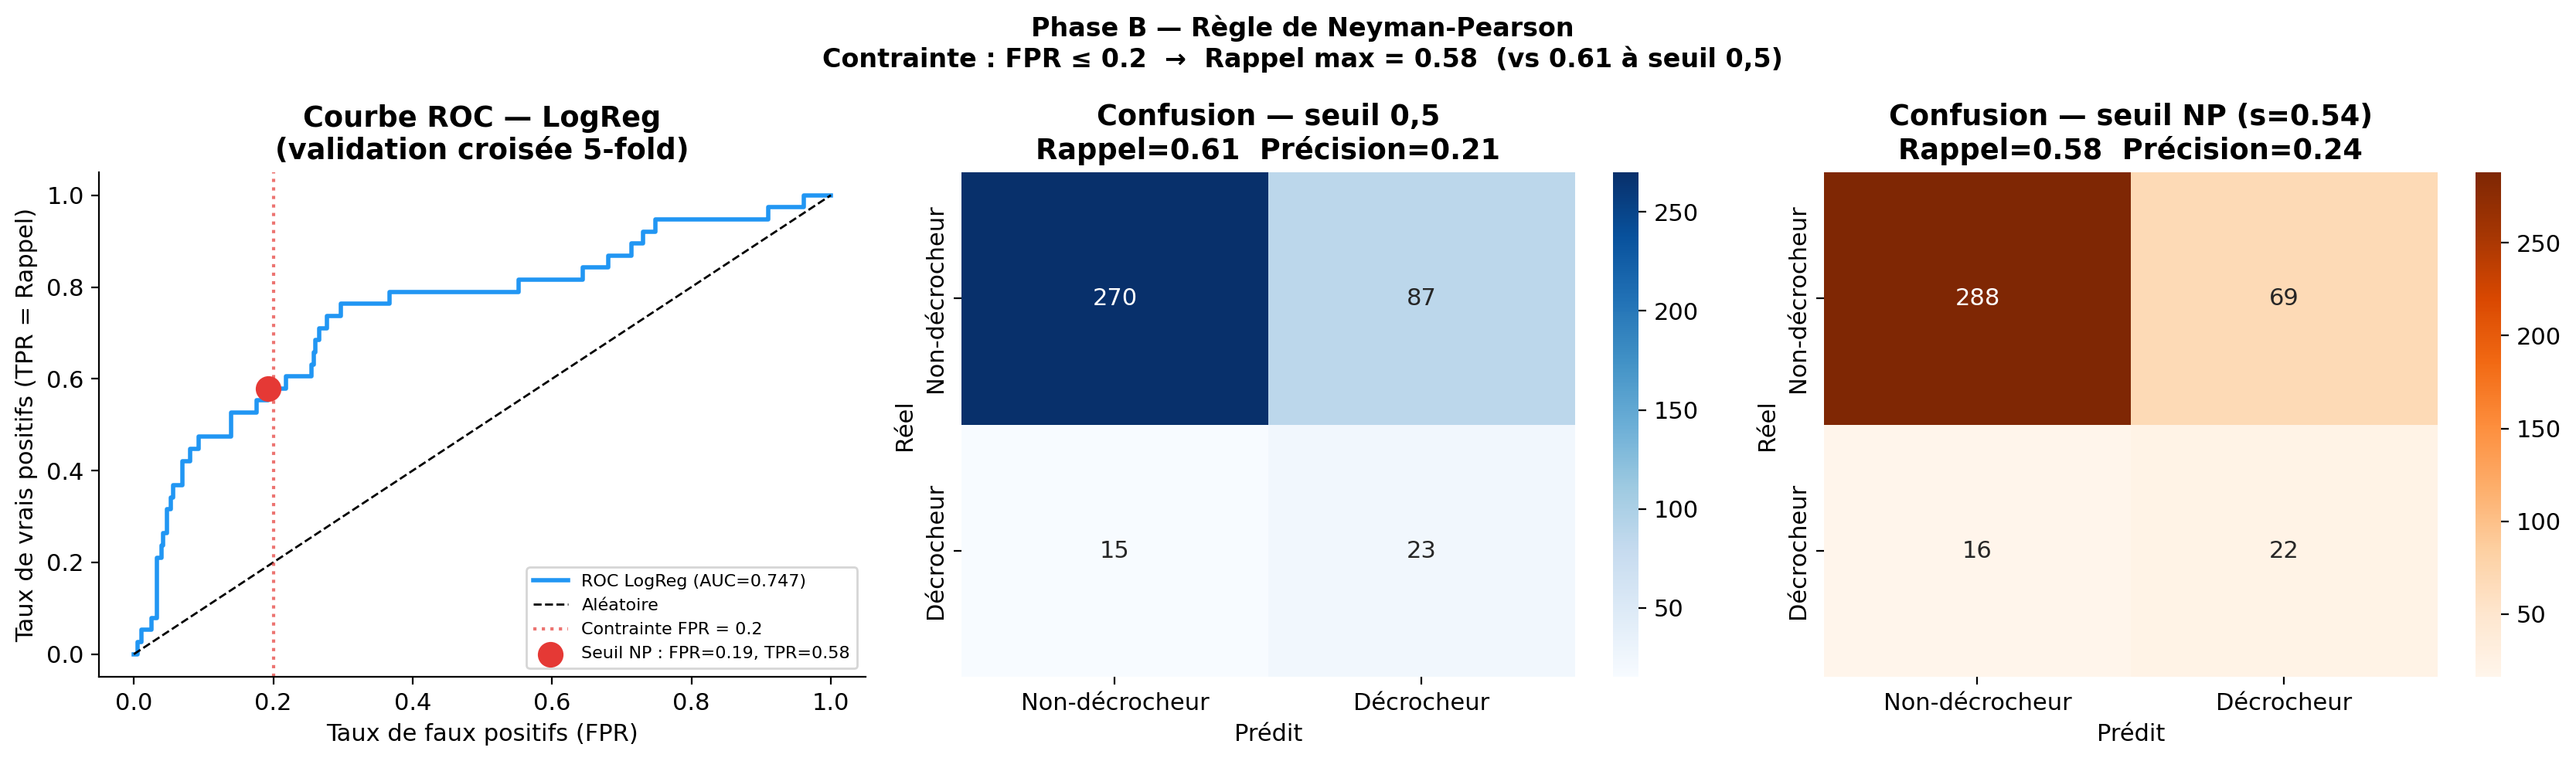
\includegraphics[width=0.92\textwidth]{02_phase_b_roc_np.png}
\caption{Régression logistique~: courbe ROC et règle de Neyman-Pearson ($\alpha^*=0{,}20$).}
\label{fig:ann_roc}
\end{figure}
\clearpage

\bibliographystyle{plain}
\bibliography{references}

\end{document}
